\chapter{Biomolecules: Amino Acids, Sugars, Lipids and Nucleotides}\label{ch:b2:biomolecules}

A common sweetener, far sweeter than sugar, is two amino acids joined by a single amide bond, one of
them as its methyl ester: aspartic acid and phenylalanine, both with the configuration living cells
use. The molecules of life are built from a few families of small units, amino acids, sugars, \omterm{def:b2:biomolecules:lipid}{fatty
acids} and \omterm{def:b2:biomolecules:nucleotide}{nucleotides}, joined by the reactions of the previous chapters: amides, acetals, esters. This
chapter reads them as an organic chemist does: functional groups, stereochemistry, acid--base
behaviour, and the reactions that join and cut them.
% ledger: use:aspartame

\begin{recall}
The Year 1 volume: CIP rules, Fischer projections, chirality, hemiacetals and acetals, $\mathrm pK_a$
and distribution diagrams, amphiphilic molecules, Biot's law. \Cref{ch:b2:acyl-substitution}: amides,
esters, \omterm{def:b2:acyl-substitution:saponification}{saponification}, activated acids. \Cref{ch:b2:amines}: amines as bases.
\Cref{ch:b2:retrosynthesis}: protecting groups in a route.
\end{recall}

\section{Amino acids}

\begin{definition}[Amino acids]\label{def:b2:biomolecules:amino-acid}
An \emph{$\alpha$-amino acid}\index{alpha-amino acid@$\alpha$-amino acid} \ce{H2N-CHR-COOH} carries an
amino group and a carboxylic acid group on the same carbon; \ce{R} is its \emph{side
chain}\index{side chain}. In water near neutral pH it exists as a \emph{zwitterion}\index{zwitterion},
\ce{H3N+-CHR-COO-}, carrying a positive and a negative charge. The \emph{isoelectric
point}\index{isoelectric point} pI is the pH at which its average net charge is zero.
\end{definition}

Twenty amino acids build the proteins of living things. All but glycine (\ce{R = H}) are chiral, and
the natural ones have the L configuration (\cref{def:b2:biomolecules:d-l}). Their \omterm{def:b2:biomolecules:amino-acid}{side chains} sort them
into families: nonpolar (alanine, \ce{R = CH3}; phenylalanine, \ce{R = CH2C6H5}), polar, acidic
(aspartic and glutamic acids, with a second carboxylic group) and basic (lysine, with a second amino
group; histidine, with an imidazole ring).

\begin{proposition}[Isoelectric point]\label{prop:b2:biomolecules:pi}
For an amino acid with a \omterm{def:b2:biomolecules:amino-acid}{side chain} that is neither acidic nor basic, $\mathrm{pI} = (\mathrm pK_{a1} +
\mathrm pK_{a2})/2$, where $\mathrm pK_{a1}$ belongs to the carboxylic group and $\mathrm pK_{a2}$ to the
ammonium group. For an acidic or basic \omterm{def:b2:biomolecules:amino-acid}{side chain}, pI is the mean of the two $\mathrm pK_a$ that frame the
neutral form.
\end{proposition}

\begin{proof}
Write \ce{H2A+} for the cation, \ce{HA} for the \omterm{def:b2:biomolecules:amino-acid}{zwitterion} and \ce{A-} for the anion. The net charge is
zero when $[\ce{H2A+}] = [\ce{A-}]$. From $K_{a1} = [\ce{HA}]h/[\ce{H2A+}]$ and $K_{a2} =
[\ce{A-}]h/[\ce{HA}]$, with $h = [\ce{H3O+}]$, the ratio $[\ce{H2A+}]/[\ce{A-}] = h^2/(K_{a1}K_{a2})$
equals 1 for $h^2 = K_{a1}K_{a2}$, that is $\mathrm{pH} = (\mathrm pK_{a1} + \mathrm pK_{a2})/2$. With a
third ionisable group the same argument applies to the two equilibria on either side of the neutral
form, the third group being then entirely in one state.
\end{proof}

For glycine, $\mathrm pK_{a1} = 2.35$ and $\mathrm pK_{a2} = 9.78$: pI $\approx 6.1$. Aspartic acid
(2.0, 3.9, 9.9) has pI $\approx 3.0$; lysine (2.2, 9.1, 10.7) has pI $\approx 9.9$.
% ledger: pka:glycine1, pka:glycine2, pka:asp1, pka:asp2, pka:asp3, pka:lys1, pka:lys2, pka:lys3

\begin{omfigure}
\begin{tikzpicture}
\begin{axis}[width=0.47\linewidth, height=5cm, xmin=0, xmax=14, ymin=-2.2, ymax=2.2,
  xlabel={pH}, ylabel={net charge}, label style={font=\small}, tick label style={font=\scriptsize},
  xtick={0,2,4,6,8,10,12,14}, ytick={-2,-1,0,1,2}, grid=major, grid style={black!12},
  legend style={font=\scriptsize, at={(0.5,1.03)}, anchor=south}, legend columns=3]
\addplot[omDef, thick] table[x=pH, y=gly] {figdata/out/bachelor-2-amino-acid-charge-a.dat};
\addplot[omThm, thick] table[x=pH, y=asp] {figdata/out/bachelor-2-amino-acid-charge-a.dat};
\addplot[omMeth, thick] table[x=pH, y=lys] {figdata/out/bachelor-2-amino-acid-charge-a.dat};
\legend{glycine, aspartic acid, lysine}
\end{axis}
\end{tikzpicture}\hfill
\begin{tikzpicture}
\begin{axis}[width=0.47\linewidth, height=5cm, xmin=0, xmax=14, ymin=0, ymax=1.05,
  xlabel={pH}, ylabel={fraction}, label style={font=\small}, tick label style={font=\scriptsize},
  xtick={0,2,4,6,8,10,12,14},
  legend style={font=\scriptsize, at={(0.5,1.03)}, anchor=south}, legend columns=3]
\addplot[omThm, thick] table[x=pH, y=cation] {figdata/out/bachelor-2-amino-acid-charge-b.dat};
\addplot[omDef, thick] table[x=pH, y=zwitterion] {figdata/out/bachelor-2-amino-acid-charge-b.dat};
\addplot[omMeth, thick] table[x=pH, y=anion] {figdata/out/bachelor-2-amino-acid-charge-b.dat};
\legend{cation, zwitterion, anion}
\end{axis}
\end{tikzpicture}

{\small Left: net charge of three amino acids against pH, from their $\mathrm pK_a$ at
\qty{25}{\degreeCelsius}; each curve crosses zero at the pI. Right: the three forms of glycine,
\ce{H3N+CH2COOH}, \ce{H3N+CH2COO-} and \ce{H2NCH2COO-}; the \omterm{def:b2:biomolecules:amino-acid}{zwitterion} dominates from about pH 3 to
pH 9.}
% figdata: bachelor-2/amino-acid-charge.py parts a, b
\end{omfigure}

\begin{method}[Net charge at a given pH]\label{met:b2:biomolecules:charge}
\begin{enumerate}
  \item List every ionisable group with its $\mathrm pK_a$: the terminal \ce{NH3+} and \ce{COOH}, and the
        ionisable \omterm{def:b2:biomolecules:amino-acid}{side chains}.
  \item For each group, compare pH and $\mathrm pK_a$: a group is mostly protonated below its
        $\mathrm pK_a$, mostly deprotonated above (by more than 1 unit: over 90~\%).
  \item Add the charges: \ce{NH3+} $+1$, \ce{NH2} 0, \ce{COOH} 0, \ce{COO-} $-1$ (imidazolium $+1$).
  \item Near a $\mathrm pK_a$, count that group as half charged; for an exact value, use the fractions
        $1/(1 + 10^{\mathrm pK_a - \mathrm{pH}})$.
\end{enumerate}
\end{method}

\section{Peptides}

\begin{definition}[Peptides]\label{def:b2:biomolecules:peptide}
The amide bond formed between the carboxylic group of one amino acid and the amino group of another is
a \emph{peptide bond}\index{peptide bond}; a chain of amino acids joined by peptide bonds is a
\emph{peptide}\index{peptide} (a protein when it is long), written from its free amino end (N-terminus)
to its free carboxylic end (C-terminus). A \emph{peptide coupling}\index{peptide coupling} forms a
peptide bond in the laboratory with a \emph{coupling agent}\index{coupling agent}, a reagent that
converts the carboxylic group into an activated derivative under mild conditions (a carbodiimide, for
instance).
\end{definition}

\begin{omfigure}
\setchemfig{atom sep=1.9em}
\schemestart
\chemfig{R-C(=[2]O)-N(-[6]H)-R'}
\arrow{<->}
\chemfig{R-C(-[2]\chemabove{O}{\scriptstyle -})=\chemabove{N}{\scriptstyle +}(-[6]H)-R'}
\schemestop
\par\vspace{6pt}

{\small The two resonance structures of the \omterm{def:b2:biomolecules:peptide}{peptide bond}. The nitrogen lone pair is shared with the
carbonyl: the \ce{C-N} bond has a partial double-bond character, and the six atoms C, C, O, N, H, C lie
in one plane.}
\end{omfigure}

\begin{proposition}[A planar bond]\label{prop:b2:biomolecules:planar}
The \omterm{def:b2:biomolecules:peptide}{peptide bond} is planar, rotation about the \ce{C-N} bond is restricted, and the amide nitrogen is
neither basic nor nucleophilic.
\end{proposition}

\begin{proof}[Argument]
The second resonance structure gives the \ce{C-N} bond a share of double-bond character: rotating it
would break the overlap of the nitrogen lone pair with the \ce{C=O} $\pi$ system, which costs energy, so
the atoms around it stay in one plane, the trans arrangement (the two chain carbons on opposite sides of
the \ce{C-N} bond) being the usual one. The lone pair engaged in the resonance is not available for a proton or an
electrophile, as for every amide (\cref{ch:b2:acyl-substitution}). Proteins fold around chains of these
rigid planes.
\end{proof}

\begin{proposition}[Why protect and activate]\label{prop:b2:biomolecules:coupling}
Making one given dipeptide from two amino acids needs both the protection of the groups that must not
react and the activation of the carboxylic group that must.
\end{proposition}

\begin{proof}[Argument]
A carboxylic acid and an amine mixed at room temperature give a salt, not an amide; heating to drive off
water would also racemise the amino acids. Activation (an \omterm{def:b2:acyl-substitution:derivative}{acyl chloride}, an anhydride, or a \omterm{def:b2:biomolecules:peptide}{coupling
agent}) is therefore needed. But each amino acid has both groups: activating a mixture of glycine and
alanine would give Gly--Ala, Ala--Gly, Gly--Gly, Ala--Ala and longer chains. Blocking the amine of the
first and the acid of the second leaves only one possible bond.
\end{proof}

\begin{method}[Synthesis of a dipeptide]\label{met:b2:biomolecules:peptide}
\begin{enumerate}
  \item Protect the amino group of the N-terminal amino acid (as a carbamate, for instance a
        \textit{tert}-butoxycarbonyl group).
  \item Protect the carboxylic group of the C-terminal amino acid (as a methyl or benzyl ester), and any
        reactive \omterm{def:b2:biomolecules:amino-acid}{side chain}.
  \item Activate the free carboxylic group with a \omterm{def:b2:biomolecules:peptide}{coupling agent} and add the protected partner: one
        \omterm{def:b2:biomolecules:peptide}{peptide bond} forms.
  \item Remove the protecting groups, preferably an orthogonal set
        (\cref{def:b2:retrosynthesis:orthogonal}); to go on, remove only the amine protection and repeat.
\end{enumerate}
\end{method}

Repeating the cycle many times in solution would need a purification at each step. In solid-phase
synthesis, the growing chain is attached by its C-terminus to a \omterm{def:b2:polymer-synthesis:polymer}{polymer} bead; excess reagents and
by-products are washed away after each coupling, and the finished \omterm{def:b2:biomolecules:peptide}{peptide} is cut from the support at
the end.

\begin{omfigure}
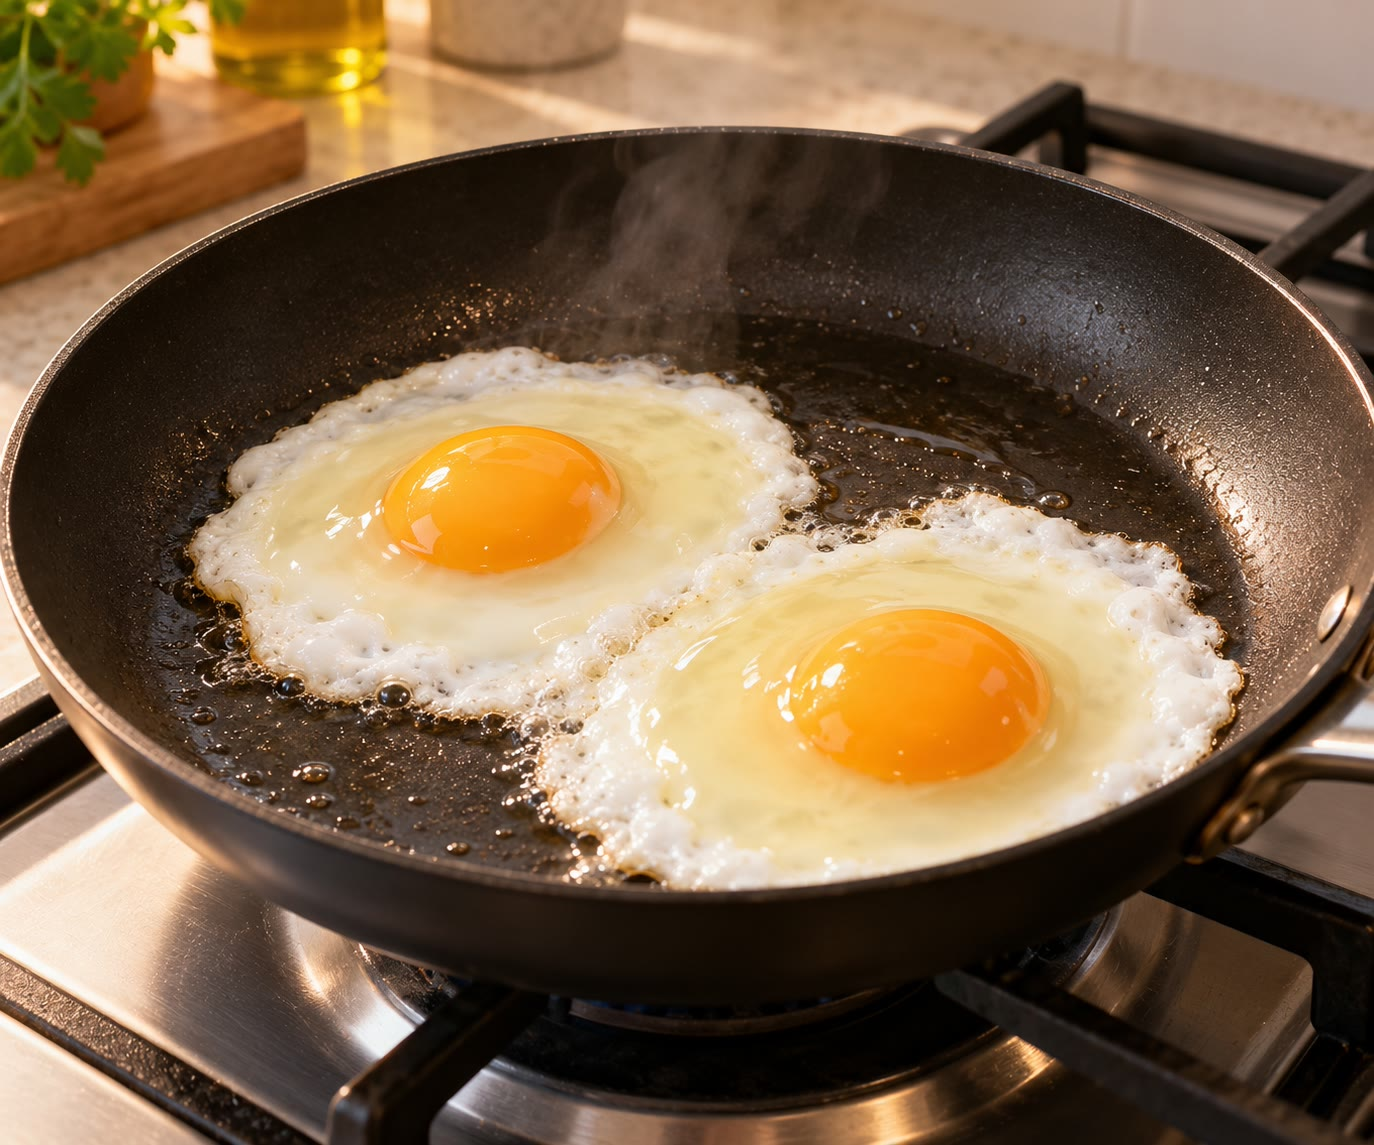
\includegraphics[width=0.5\linewidth]{images/book3/ai/b2-30-eggs.jpg}

{\small Eggs frying. The proteins of the white unfold on heating and bond to one another: the
translucent liquid turns into an opaque white solid. No \omterm{def:b2:biomolecules:peptide}{peptide bond} breaks; the change is in the way
the chains are folded (illustration).}
\end{omfigure}

\section{Carbohydrates}

\begin{definition}[D and L]\label{def:b2:biomolecules:d-l}
A sugar or an amino acid is drawn in Fischer projection with its most oxidised carbon at the top. It is
D if the \ce{OH} on the stereocentre farthest from the top (or, for an $\alpha$-amino acid, the
\ce{NH2} on the $\alpha$ carbon) points to the right, and L if it points to the left. The descriptors
compare configurations with that of glyceraldehyde; they are not the CIP descriptors.
\end{definition}

\begin{definition}[Monosaccharides]\label{def:b2:biomolecules:sugar}
A \emph{monosaccharide}\index{monosaccharide} is a polyhydroxy aldehyde or ketone, usually
\ce{C_nH_{2n}O_n} with $n$ from 3 to 7, that cannot be hydrolysed into smaller sugars. An
\emph{aldose}\index{aldose} has an aldehyde group at C1, a \emph{ketose}\index{ketose} a ketone group,
usually at C2. Glucose is an aldohexose, fructose a ketohexose.
\end{definition}

In water an aldohexose is almost entirely cyclic: the \ce{OH} on C5 adds to the aldehyde, forming a
six-membered hemiacetal ring (a pyranose). The cyclisation creates a new stereocentre at C1.

\begin{definition}[Anomers]\label{def:b2:biomolecules:anomer}
In a \emph{Haworth projection}\index{Haworth projection} the ring of a cyclic sugar is drawn flat,
perpendicular to the page, with its oxygen at the back right and its substituents above or below the
ring. The hemiacetal carbon (C1 of an \omterm{def:b2:biomolecules:sugar}{aldose}) is the \emph{anomeric carbon}\index{anomeric carbon}; the
two configurations it can take give two diastereoisomers, the \emph{anomers}\index{anomers}: for a D
sugar, $\alpha$ has the anomeric \ce{OH} below the ring (opposite the \ce{CH2OH}), $\beta$ above. In
water the anomers interconvert through the open chain, and the optical rotation of a freshly dissolved
anomer drifts to an equilibrium value: \emph{mutarotation}\index{mutarotation}.
\end{definition}

\begin{omfigure}
\setchemfig{atom sep=1.7em}
\begin{minipage}[c]{0.24\linewidth}\centering
\chemfig{CHO-[6]C(-[4]H)(-[0]OH)-[6]C(-[4,,,2]HO)(-[0]H)-[6]C(-[4]H)(-[0]OH)-[6]C(-[4]H)(-[0]OH)-[6]CH_2OH}
\end{minipage}%
\begin{minipage}[c]{0.37\linewidth}\centering
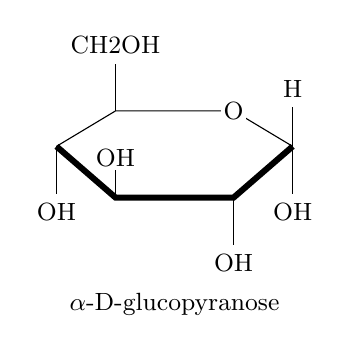
\begin{tikzpicture}[x=1cm, y=1cm, font=\small]
\coordinate (C4) at (-1.5,0); \coordinate (C3) at (-0.75,-0.65); \coordinate (C2) at (0.75,-0.65);
\coordinate (C1) at (1.5,0); \coordinate (O) at (0.75,0.45); \coordinate (C5) at (-0.75,0.45);
\draw (C5) -- (O) -- (C1); \draw (C4) -- (C5);
\draw[line width=2.2pt] (C4) -- (C3) -- (C2) -- (C1);
\node[fill=white, inner sep=1pt] at (O) {O};
\draw (C5) -- ++(0,0.6) node[above] {\ce{CH2OH}};
\draw (C1) -- ++(0,-0.6) node[below] {OH}; \draw (C1) -- ++(0,0.5) node[above] {H};
\draw (C2) -- ++(0,-0.6) node[below] {OH}; \draw (C3) -- ++(0,0.35) node[above, inner sep=1pt] {OH};
\draw (C4) -- ++(0,-0.6) node[below] {OH};
\node at (0,-2.0) {$\alpha$-D-glucopyranose};
\end{tikzpicture}
\end{minipage}%
\begin{minipage}[c]{0.37\linewidth}\centering
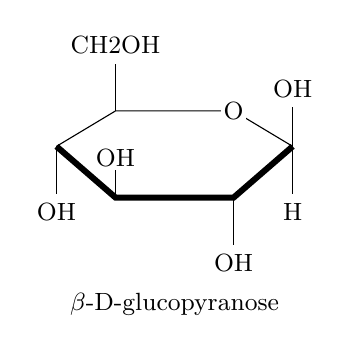
\begin{tikzpicture}[x=1cm, y=1cm, font=\small]
\coordinate (C4) at (-1.5,0); \coordinate (C3) at (-0.75,-0.65); \coordinate (C2) at (0.75,-0.65);
\coordinate (C1) at (1.5,0); \coordinate (O) at (0.75,0.45); \coordinate (C5) at (-0.75,0.45);
\draw (C5) -- (O) -- (C1); \draw (C4) -- (C5);
\draw[line width=2.2pt] (C4) -- (C3) -- (C2) -- (C1);
\node[fill=white, inner sep=1pt] at (O) {O};
\draw (C5) -- ++(0,0.6) node[above] {\ce{CH2OH}};
\draw (C1) -- ++(0,0.5) node[above] {OH}; \draw (C1) -- ++(0,-0.6) node[below] {H};
\draw (C2) -- ++(0,-0.6) node[below] {OH}; \draw (C3) -- ++(0,0.35) node[above, inner sep=1pt] {OH};
\draw (C4) -- ++(0,-0.6) node[below] {OH};
\node at (0,-2.0) {$\beta$-D-glucopyranose};
\end{tikzpicture}
\end{minipage}
\par\vspace{6pt}

{\small D-Glucose. Left: the open chain in Fischer projection, \ce{OH} on C5 to the right (D). Middle
and right: the two pyranose \omterm{def:b2:biomolecules:anomer}{anomers} in \omterm{def:b2:biomolecules:anomer}{Haworth projection}; the groups on the right of the Fischer
projection point down, those on the left point up, and C5 carries the \ce{CH2OH} up. The \omterm{def:b2:biomolecules:anomer}{anomers}
differ only at C1. Hydrogens on C2 to C5 are omitted.}
\end{omfigure}

\begin{method}[From Fischer to Haworth (D-aldopyranose)]\label{met:b2:biomolecules:haworth}
\begin{enumerate}
  \item Draw the ring with O at the back right, C1 at the right, then C2, C3, C4 clockwise along the
        front and left, C5 at the back left.
  \item Groups on the right in the Fischer projection go down, groups on the left go up.
  \item On C5 (D series), the \ce{CH2OH} goes up.
  \item On C1, the \ce{OH} goes down for $\alpha$, up for $\beta$.
\end{enumerate}
\end{method}

\begin{proposition}[Mutarotation equilibrium]\label{prop:b2:biomolecules:mutarotation}
If the specific rotations of the pure \omterm{def:b2:biomolecules:anomer}{anomers} are $[\alpha]_\alpha$ and $[\alpha]_\beta$ and that of the
equilibrium mixture is $[\alpha]_{\mathrm{eq}}$, the mole fraction of the $\alpha$ anomer at
equilibrium is
\begin{equation*}
x_\alpha = \frac{[\alpha]_{\mathrm{eq}} - [\alpha]_\beta}{[\alpha]_\alpha - [\alpha]_\beta}.
\end{equation*}
\end{proposition}

\begin{proof}
The open chain is a tiny fraction of the mixture and is neglected. The rotations of the two \omterm{def:b2:biomolecules:anomer}{anomers}
add in proportion to their concentrations (Biot's law, Year 1 volume); since they have the same molar
mass, $[\alpha]_{\mathrm{eq}} = x_\alpha[\alpha]_\alpha + (1 - x_\alpha)[\alpha]_\beta$, which is solved
for $x_\alpha$.
\end{proof}

D-Glucose at equilibrium in water has $[\alpha] = +52.7$ (in \unit{\degree\,dm^{-1}\,g^{-1}\,mL}).
With anomer rotations of $+112$ and $+18.7$ (exercise data), $x_\alpha = (52.7 - 18.7)/(112 - 18.7)
\approx 0.36$: about 36~\% $\alpha$ and 64~\% $\beta$. The $\beta$ anomer, with all its
substituents equatorial in the chair, is the more stable.
% ledger: rot:glucose-eq

\begin{definition}[Glycosides]\label{def:b2:biomolecules:glycoside}
A \emph{glycoside}\index{glycoside} is the acetal formed when the anomeric \ce{OH} of a sugar is replaced
by an \ce{OR} group from an alcohol, often another sugar; the bond from the \omterm{def:b2:biomolecules:anomer}{anomeric carbon} to that
oxygen is the \emph{glycosidic bond}\index{glycosidic bond}. A \emph{reducing sugar}\index{reducing sugar}
is one that reduces mild oxidants such as Fehling's solution or Tollens' reagent.
\end{definition}

\begin{proposition}[Reducing or not]\label{prop:b2:biomolecules:reducing}
A sugar with a free hemiacetal (or hemiketal) group is reducing; a \omterm{def:b2:biomolecules:glycoside}{glycoside} whose \omterm{def:b2:biomolecules:anomer}{anomeric carbons} are
all engaged in \omterm{def:b2:biomolecules:glycoside}{glycosidic bonds} is not.
\end{proposition}

\begin{proof}[Argument]
A hemiacetal is in equilibrium with the open chain, whose aldehyde group is oxidised by the reagent;
the equilibrium then reopens more rings until all the sugar has reacted. An acetal does not open in
neutral or basic water: the \omterm{def:b2:biomolecules:anomer}{anomeric carbon} stays locked, with no aldehyde to oxidise.
\end{proof}

Maltose (two glucoses, C1 of one bonded to O4 of the other) keeps one free hemiacetal and is reducing;
sucrose joins the \omterm{def:b2:biomolecules:anomer}{anomeric carbons} of glucose and fructose to each other and is not. Starch and
cellulose are both chains of glucose joined C1--O4: $\alpha$ in starch, which coils and is digested;
$\beta$ in cellulose, whose straight chains pack into fibres held by hydrogen bonds.

\section{Lipids}

\begin{definition}[Lipids]\label{def:b2:biomolecules:lipid}
A \emph{fatty acid}\index{fatty acid} is a carboxylic acid with a long unbranched chain, usually of 12 to
22 carbons, saturated or with (\textit{Z}) double bonds. A \emph{triglyceride}\index{triglyceride} is the
triester of propane-1,2,3-triol (glycerol) with three fatty acids. A
\emph{phospholipid}\index{phospholipid} is a diester of glycerol with two fatty acids whose third
position carries a phosphate group bonded to a small polar group.
\end{definition}

The (\textit{Z}) double bonds bend the chains, which then pack badly: stearic acid (18 carbons,
saturated) melts at \qty{69}{\degreeCelsius}, oleic acid (18 carbons, one \textit{Z} double bond) at
\qty{13}{\degreeCelsius}. Fats rich in saturated chains are solid at room temperature; oils, rich in
unsaturated chains, are liquid. \omterm{def:b2:biomolecules:lipid}{Triglycerides} are saponified into glycerol and soaps
(\cref{ch:b2:acyl-substitution}).
% ledger: mp:stearic, mp:oleic

\begin{omfigure}
\begin{tikzpicture}[x=1cm, y=1cm]
\foreach \i in {0,1,2,3,4,5,6,7,8,9}{
  \fill[omDef!60] (0.6*\i,1.6) circle (0.17);
  \draw[thick, black!70] (0.6*\i-0.06,1.43) .. controls (0.6*\i-0.12,1.2) and (0.6*\i,1.0) .. (0.6*\i-0.06,0.75);
  \draw[thick, black!70] (0.6*\i+0.06,1.43) .. controls (0.6*\i+0.12,1.2) and (0.6*\i,1.0) .. (0.6*\i+0.06,0.75);
  \fill[omDef!60] (0.6*\i,-0.6) circle (0.17);
  \draw[thick, black!70] (0.6*\i-0.06,-0.43) .. controls (0.6*\i-0.12,-0.2) and (0.6*\i,0.0) .. (0.6*\i-0.06,0.25);
  \draw[thick, black!70] (0.6*\i+0.06,-0.43) .. controls (0.6*\i+0.12,-0.2) and (0.6*\i,0.0) .. (0.6*\i+0.06,0.25);
}
\node[font=\small, anchor=west] at (6.0,2.2) {water};
\node[font=\small, anchor=west] at (6.0,0.5) {hydrocarbon core};
\node[font=\small, anchor=west] at (6.0,-1.2) {water};
\draw[densely dotted] (5.6,1.6) -- (6.0,1.6) node[right, font=\footnotesize] {polar heads};
\draw[densely dotted] (5.6,1.05) -- (6.0,1.05) node[right, font=\footnotesize] {two fatty-acid tails};
\end{tikzpicture}
\par\vspace{4pt}

{\small A \omterm{def:b2:biomolecules:lipid}{phospholipid} bilayer, schematic: the polar heads face the water on both sides, the
hydrocarbon tails meet inside. Cell membranes are built on this structure; soaps, with one tail per
head, form instead small spheres with the tails inside, called micelles.}
\end{omfigure}

\section{Nucleotides}

\begin{definition}[Nucleotides]\label{def:b2:biomolecules:nucleotide}
A \emph{nucleobase}\index{nucleobase} is a nitrogen heterocycle: adenine (A) and guanine (G), purines;
cytosine (C), thymine (T) and uracil (U), pyrimidines. A \emph{nucleoside}\index{nucleoside} is a
nucleobase bonded by a nitrogen to C1 of ribose or 2-deoxyribose (an $N$-glycoside). A
\emph{nucleotide}\index{nucleotide} is a phosphate ester of a nucleoside. In nucleic acids the
nucleotides are joined by \emph{phosphodiester bonds}\index{phosphodiester bond}: one phosphate links
O3 of one sugar to O5 of the next.
\end{definition}

DNA uses 2-deoxyribose and the bases A, G, C, T; RNA uses ribose and U in place of T. The chain has a
direction, from its 5$'$ end to its 3$'$ end, and the phosphates, ionised at physiological pH, make it a
polyanion. Two DNA strands run in opposite directions and are held together by hydrogen bonds between
bases facing each other.

\begin{proposition}[Base pairing]\label{prop:b2:biomolecules:pairing}
In double-stranded DNA, adenine pairs with thymine through two hydrogen bonds, and guanine with cytosine
through three.
\end{proposition}

\begin{proof}[Argument]
The pairs are those whose edges match donors (\ce{N-H}) with acceptors (\ce{C=O} oxygen, ring
nitrogen) at the right distances, with a purine facing a pyrimidine so that every pair has the same
width. A offers \ce{N-H} (its amino group) and a ring \ce{N}; T offers \ce{C=O} and \ce{N-H}: two bonds. G
offers \ce{C=O}, \ce{N-H} and \ce{N-H} (amino); C offers \ce{N-H} (amino), \ce{N} and \ce{C=O}: three
bonds. The figure shows them.
\end{proof}

\begin{omfigure}
\setchemfig{atom sep=1.7em}
\chemfig{?[a](-[:90]CH_3)-[:-30](=[:30]@{to}O)-[:-90]N(-[:-30]@{th}H)-[:-150](=[:-90]O)-[:150]N(-[:-150]R)-[:90]?[a,2]}%
\hspace{2.3em}%
\raisebox{-1.0em}{\chemfig{?[a](-[:150]N(-[:90]H)-[:210]@{ah}H)-[:30]?[b](-[:78]N=[:6]-[:-66]N(-[:-30]R)-[:-138]?[c])=[:-30]?[c]-[:-90]N=[:-150]-[:150]@{an}N?[a,2]}}
\chemmove{\draw[-, densely dotted, thick](to)--(ah); \draw[-, densely dotted, thick](th)--(an);}
\hspace{1.5em}
\chemfig{?[a]-[:-30](-[:30]N(-[:90]H)-[:-30]@{ch}H)=[:-90]@{cn}N-[:-150](=[:-90]@{co}O)-[:150]N(-[:-150]R)-[:90]?[a,2]}%
\hspace{2.3em}%
\raisebox{-0.6em}{\chemfig{?[a](=[:150]@{go}O)-[:30]?[b](-[:78]N=[:6]-[:-66]N(-[:-30]R)-[:-138]?[c])=[:-30]?[c]-[:-90]N=[:-150](-[:-90]N(-[:-30]H)-[:-150]@{gh}H)-[:150]N?[a](-[:180]@{gn}H)}}
\chemmove{\draw[-, densely dotted, thick](ch)--(go); \draw[-, densely dotted, thick](cn)--(gn);
  \draw[-, densely dotted, thick](co)--(gh);}
\par\vspace{6pt}

{\small The two base pairs of DNA. Left: thymine and adenine, two hydrogen bonds (dotted). Right:
cytosine and guanine, three. R is the deoxyribose of each strand; the two R groups of a pair point to
the same side, towards the two backbones.}
\end{omfigure}

\begin{history}[The sugars, 1891]
\begin{minipage}[t]{0.18\linewidth}
\vspace{0pt}
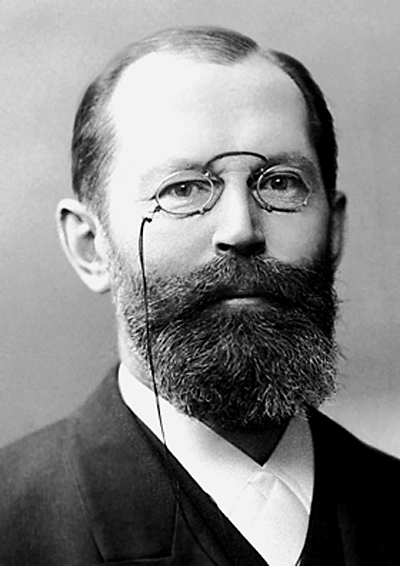
\includegraphics[width=\linewidth]{images/book3/fischer.jpg}
\end{minipage}\hfill
\begin{minipage}[t]{0.78\linewidth}
\vspace{0pt}
Emil Fischer worked out, by 1891, the configurations of glucose and of its isomers, before any
physical method could see a molecule: by converting sugars into one another and counting the
stereoisomers obtained. The projection he invented to write them still bears his name. He also made
the first synthetic \omterm{def:b2:biomolecules:peptide}{peptides}, and received the 1902 Nobel Prize in Chemistry. (Portrait: Atelier
Victoria, Berlin, around 1895, public domain; Wikimedia Commons.)
\end{minipage}
\end{history}

\section{Exercises}

\begin{exercise}[$\star$]\label{exo:b2:biomolecules:1}
Draw alanine as a \omterm{def:b2:biomolecules:amino-acid}{zwitterion}, then the forms that dominate at pH 1 and at pH 12.
\end{exercise}

\begin{exercise}[$\star$]\label{exo:b2:biomolecules:2}
Compute the \omterm{def:b2:biomolecules:amino-acid}{isoelectric point} of glycine, and that of alanine ($\mathrm pK_a$ 2.35 and 9.87).
\end{exercise}

\begin{exercise}[$\star$]\label{exo:b2:biomolecules:3}
Draw the dipeptide Ala--Gly and circle its \omterm{def:b2:biomolecules:peptide}{peptide bond}. How does it differ from Gly--Ala?
\end{exercise}

\begin{exercise}[$\star$]\label{exo:b2:biomolecules:4}
In a Fischer projection with \ce{COOH} at the top and the \omterm{def:b2:biomolecules:amino-acid}{side chain} \ce{CH2OH} at the bottom, the
\ce{NH2} of serine points to the left. Is it D or L? Give its CIP descriptor.
\end{exercise}

\begin{exercise}[$\star\star$]\label{exo:b2:biomolecules:5}
Give the net charge of the tripeptide Lys--Gly--Asp at pH 1, 7 and 12.
\end{exercise}

\begin{exercise}[$\star\star$]\label{exo:b2:biomolecules:6}
Why is a \omterm{def:b2:biomolecules:peptide}{coupling agent} used to make a \omterm{def:b2:biomolecules:peptide}{peptide bond}, rather than an \omterm{def:b2:acyl-substitution:derivative}{acyl chloride} of the protected amino
acid made with thionyl chloride and heated?
\end{exercise}

\begin{exercise}[$\star\star$]\label{exo:b2:biomolecules:7}
D-Fructose cyclises through its C5 \ce{OH} onto the C2 ketone. Give the size of the ring and draw
$\beta$-D-fructofuranose in \omterm{def:b2:biomolecules:anomer}{Haworth projection}.
\end{exercise}

\begin{exercise}[$\star\star$]\label{exo:b2:biomolecules:8}
The pure \omterm{def:b2:biomolecules:anomer}{anomers} of D-galactose have specific rotations of $+150.7$ ($\alpha$) and $+52.8$ ($\beta$) and
the equilibrium mixture $+80.2$ (exercise data). Compute the equilibrium composition.
\end{exercise}

\begin{exercise}[$\star\star$]\label{exo:b2:biomolecules:9}
Explain why maltose reduces Fehling's solution and sucrose does not, and why sucrose does after
heating with dilute acid.
\end{exercise}

\begin{exercise}[$\star\star\star$]\label{exo:b2:biomolecules:10}
The \omterm{def:b2:acyl-substitution:saponification}{saponification} value of a fat is the mass of potassium hydroxide, in mg, that saponifies 1~g of it.
Compute it for triolein, \ce{C57H104O6}, and explain why a fat with shorter chains has a higher value.
\end{exercise}

\begin{exercise}[$\star\star\star$]\label{exo:b2:biomolecules:11}
Plan the synthesis of Gly--Ala from glycine and alanine: protecting groups, activation, coupling,
deprotection, with an orthogonal pair.
\end{exercise}

\begin{exercise}[$\star\star\star$]\label{exo:b2:biomolecules:12}
Write the strand complementary to 5$'$-ATGCGT-3$'$, from its 5$'$ end, and count the hydrogen bonds
that hold the double strand together.
\end{exercise}

\section{Problem: Aspartame}

\begin{problem}[{Weekend problem --- the two amino acids and their configurations, the charge of the
dipeptide against pH, its synthesis and the $\alpha$/$\beta$ problem, and its hydrolysis in a soft
drink}]
\label{pb:b2:biomolecules:1}
Aspartame is the methyl ester of the dipeptide formed by the $\alpha$-carboxylic group of L-aspartic acid
with the amino group of L-phenylalanine. Data: $\mathrm pK_a$ of aspartic acid 2.0, 3.9 and 9.9 (model
values for the groups of the dipeptide). Molar masses (\unit{g/mol}): C 12.011, H 1.008, N 14.007,
O 15.999.
% ledger: use:aspartame, pka:asp1, pka:asp2, pka:asp3, aw:C, aw:H, aw:N, aw:O

\medskip
\noindent\textbf{Part I --- The two amino acids.}
\begin{enumerate}
  \item Name the three compounds released by the complete hydrolysis of aspartame.
  \item Draw L-aspartic acid and L-phenylalanine in Fischer projection.
  \item Give the CIP descriptor of each stereocentre.
  \item How many stereoisomers does aspartame have?
  \item Draw aspartame and mark the \omterm{def:b2:biomolecules:peptide}{peptide bond} and the ester.
  \item Why is the configuration of each amino acid important for the sweet taste?
\end{enumerate}

\medskip
\noindent\textbf{Part II --- Charge against pH.}
\begin{enumerate}[resume]
  \item List the ionisable groups of aspartame. Why is the C-terminus not one of them?
  \item With the model values, give the net charge at pH 2.
  \item The same at pH 7.
  \item The same at pH 12.
  \item Estimate the \omterm{def:b2:biomolecules:amino-acid}{isoelectric point} in this model.
  \item Why would the true $\mathrm pK_a$ values of the dipeptide differ from those of free aspartic
        acid?
\end{enumerate}

\medskip
\noindent\textbf{Part III --- Synthesis.}
\begin{enumerate}[resume]
  \item Why can aspartic acid and the methyl ester of phenylalanine not simply be heated together?
  \item Which groups of aspartic acid must be protected?
  \item What does a \omterm{def:b2:biomolecules:peptide}{coupling agent} do to the free carboxylic group?
  \item Aspartic acid has two carboxylic groups. What is formed if the wrong one is coupled?
  \item Propose an orthogonal protection that leaves only the $\alpha$-carboxylic group free, and its
        removal.
  \item Why must the activated amino acid not be left too long in basic conditions?
  \item Write the sequence of steps.
\end{enumerate}

\medskip
\noindent\textbf{Part IV --- Hydrolysis in a soft drink.}
\begin{enumerate}[resume]
  \item Which bonds of aspartame can be hydrolysed in an acidic drink? Which goes first?
  \item Give the products of the hydrolysis of the ester alone.
  \item Why does an old drink taste less sweet?
  \item Compute the molar mass of aspartame, \ce{C14H18N2O5}.
  \item Compute the amount of aspartame in a can containing \qty{180}{mg}.
  \item State the mass of methanol released by the complete hydrolysis of \qty{180}{mg} of
        aspartame.
\end{enumerate}
\end{problem}
